\documentclass[tikz,border=10pt]{standalone}
\usepackage{tikz}
\usetikzlibrary{automata, positioning, arrows.meta, bending}
\usetikzlibrary{calc}

\begin{document}
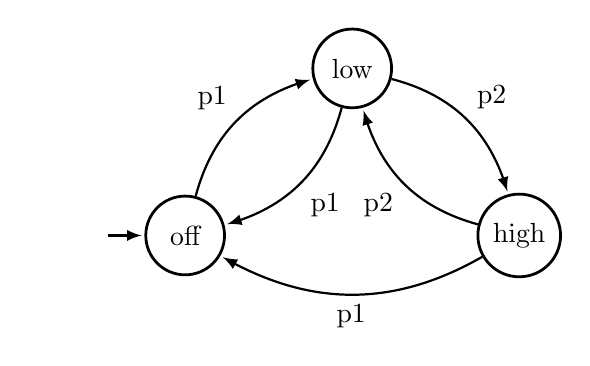
\begin{tikzpicture}[shorten >=1pt,node distance=3cm,on grid,auto,line width=1pt, every edge/.style={draw, -latex, thick},state/.style={circle, draw, minimum size=1cm}]
   \node[state] (q_1) {off};
   \node[state] (q_2) [above right=of q_1] {low};
   \node[state] (q_3) [below right=of q_2] {high};
   \node[state,draw=none] (q_4) [left = 1.5cm of q_1] {};
   
   \path[->]
   (q_1) edge[bend left] node {p1} (q_2)
   (q_2) edge[bend left] node {p1} (q_1)
   (q_2) edge[bend left] node {p2} (q_3)
   (q_3) edge[bend left] node {p1} (q_1)
   (q_3) edge[bend left] node {p2} (q_2)
   (q_4) edge node {} (q_1);
\end{tikzpicture}
\end{document}
